\documentclass[fleqn,10pt]{wlscirep}
\usepackage[utf8]{inputenc}
\usepackage[T1]{fontenc}
\usepackage{array}
\usepackage{algorithm}
\usepackage{algpseudocode}

\newcolumntype{L}[1]{>{\raggedright\arraybackslash}p{#1}}
\DeclareRobustCommand{\code}[1]{\path{#1}}
\newcommand{\RankOf}{\operatorname{rank\_of}}
\newcommand{\Tokenize}{\operatorname{tokenize}}
\newcommand{\Detokenize}{\operatorname{detokenize}}
\newcommand{\NextLogits}{\operatorname{next\_logits}}
\renewcommand{\thetable}{S\arabic{table}}
\renewcommand{\thefigure}{S\arabic{figure}}
\renewcommand{\thealgorithm}{S\arabic{algorithm}}

\title{Supplementary Information for\\
RankCloak: Measuring LLM Rank-Transcoding Steganography for Synthetic Cryptographic Artifacts}

\author[1,*]{Alexander V. Mantzaris}
\affil[1]{School of Data, Mathematical, and Statistical Sciences, University of Central Florida, Orlando, FL, United States of America}
\affil[*]{Correspondence: alexander.mantzaris@ucf.edu}

\begin{abstract}
This Supplementary Information supports the RankCloak manuscript by providing additional protocol definitions, limitation audits, detailed segmented metrics, cover-message examples, and diagnostic figures. The supplementary methods define the evaluated non-segmented and segmented protocol variants, including the experimental lead-in variant that produced one exact-recovery failure. The supplementary results expand the main manuscript's recovery, forced-span versus full-message, tail-topic, and cross-pilot interpretations under the same partial-pilot framing. The examples illustrate how deterministic synthetic hex-like payloads are mapped to bounded ranks and expressed as public cover messages with non-payload tails. The figures provide feature-only detector, effect-size, artifact, and exploratory failure-mode diagnostics. These materials are intended to aid interpretation and reproducibility; they are not additional experiments, final matrix-level inference, or evidence of cryptographic security, edit robustness, human naturalness, or undetectability.
\end{abstract}



\begin{document}
\maketitle


%%%%%%%%%%%%%%%%%%%%%%%%%%%%%
%%%%%%%%%%%%%%%%%%%%%%%%%%%%%
\section*{Supplementary Methods}

\subsection*{Protocol variants}
The main manuscript uses short labels for the protocol variants so that the Results section does not depend on repository-specific names. Supplementary Table~\ref{tab:s1} defines these labels and explains how the variants differ. The table should be read in two groups. The first three rows are non-segmented variants, where the receiver replays the complete generated cover text. The final three rows are segmented variants, where the receiver decodes only the payload-bearing forced span and ignores any non-payload tail text.

The main distinction in Supplementary Table~\ref{tab:s1} is therefore not only the payload representation, but also the part of the public message used during recovery. ASCII \(B=8\), ASCII \(B=16\), and Hex nibble differ in how they map the displayed synthetic payload into ranks, but all three use exact-copy replay of the complete cover. Seg. single topic and Seg. multi topic use hex-nibble ranks split into 8-rank chunks and decode only forced spans. Seg. lead-in adds an additional greedy lead-in before the forced span and is listed separately because it produced one exact-recovery failure in the completed partial pilot.

\begin{table}[H]
\centering
\scriptsize
\setlength{\tabcolsep}{2pt}
\begin{tabular}{L{0.12\linewidth} L{0.13\linewidth} L{0.10\linewidth} L{0.13\linewidth} L{0.13\linewidth} L{0.07\linewidth} L{0.12\linewidth} L{0.14\linewidth}}
\toprule
Variant label & Payload representation & Segmentation & Prompt schedule & Tail/filter & Lead-in & Decoder behavior & Current status \\
\midrule
ASCII \(B=8\) & ASCII-byte fixed radix & None & Ordinary prose prompts & None & None & Exact-copy replay & 8/8 completed rows recovered. \\
ASCII \(B=16\) & ASCII-byte fixed radix & None & Ordinary prose prompts & None & None & Exact-copy replay & 6/6 completed rows recovered. \\
Hex nibble & Raw hex nibbles & None & Ordinary prose prompts & None & None & Exact-copy replay & 6/6 completed rows recovered; hex-like only. \\
Seg. single topic & Raw hex nibbles & 8-rank chunks & recipe long & Sentence-boundary tail; safe-text filter & None & Forced span only & 3/3 completed rows recovered. \\
Seg. multi topic & Raw hex nibbles & 8-rank chunks & Rotating prose prompts & Sentence-boundary tail; safe-text filter & None & Forced span only & 3/3 completed rows recovered. \\
Seg. lead-in & Raw hex nibbles & 8-rank chunks & Rotating prose prompts & Sentence-boundary tail; safe-text filter & 8 greedy tokens & Replay lead-in; decode forced span & 0/1 completed row recovered; experimental. \\
\bottomrule
\end{tabular}
\caption{\label{tab:s1}Protocol variant definitions used in exploration. Decoder behavior is exact-copy replay for non-segmented rows and forced-span-only decoding for segmented rows. The Seg. lead-in variant is experimental and is not treated as a validated protocol improvement.}
\end{table}

Supplementary Table~\ref{tab:s1} is intended as a reader-facing protocol map. It is not a result table by itself, although the final column reports the completed-row recovery status to explain why the lead-in variant is handled separately. The table also motivates the later metric distinction: full-message quality metrics are straightforward for non-segmented rows, but segmented rows require separate forced-span and full-message reporting because only the forced span is decoded.

\subsection*{Experimental lead-in variant}

Supplementary Algorithm~\ref{alg:supp-leadin} defines the experimental lead-in variant. This variant was tested to ask whether a short natural-looking prefix before the forced span could make segmented messages less abrupt. Unlike the validated non-lead-in segmented variants, however, the lead-in variant requires the receiver to replay additional non-payload tokens before decoding the payload-bearing forced span. This creates an extra alignment condition: if the replayed lead-in context differs from the generation context, the ranks recovered from the forced span can change.

The algorithm is included because the lead-in variant produced the only exact-recovery failure among the completed segmented trials. It should therefore be read as a documented failure mode rather than as part of the validated protocol. The validated segmented variants begin decoding at the forced span; the lead-in variant first replays the greedy lead-in, then decodes the forced span, and finally ignores the natural tail.

\setcounter{algorithm}{0}
\begin{algorithm}[H]
\caption{Experimental lead-in segmented variant}
\label{alg:supp-leadin}
\begin{algorithmic}[1]
\Require Segment prompt \(p_j\); model \(M\); forced-rank chunk \(R_j\); lead-in length \(\ell=8\); token filter \(F\); tail policy \(T\).
\Ensure Public message with lead-in, forced span, and tail; recovered segment ranks.
\State \(\mathrm{context} \gets \Tokenize(p_j)\)
\State \(\mathrm{lead\_in} \gets [\,]\)
\For{\(k=1,\ldots,\ell\)}
    \State choose rank-1 token \(z_k\) under \(M.\NextLogits(\mathrm{context})\)
    \State append \(z_k\) to \(\mathrm{lead\_in}\) and \(\mathrm{context}\)
\EndFor
\State \(\mathrm{forced\_tokens} \gets [\,]\)
\For{each rank \(r \in R_j\)}
    \State compute logits under current context
    \State apply \(F\) to obtain allowed tokens
    \State choose token \(y\) with one-indexed rank \(r\)
    \State append \(y\) to \(\mathrm{forced\_tokens}\) and \(\mathrm{context}\)
\EndFor
\State \(\mathrm{tail} \gets \Call{GreedyTail}{M,\mathrm{context},T}\)
\State \(\mathrm{message} \gets \Detokenize(\operatorname{concat}(\mathrm{lead\_in},\mathrm{forced\_tokens},\mathrm{tail}))\)
\Statex
\State To recover, replay the same lead-in tokens one at a time, decode only the forced span, and ignore the tail.
\State \Return \(\mathrm{message}\) and recovered segment ranks
\end{algorithmic}
\end{algorithm}

Here, \(\operatorname{concat}(\cdot)\) denotes sequence concatenation. Supplementary Algorithm~\ref{alg:supp-leadin} shows why the lead-in failure is treated as a boundary-replay limitation. Adding non-payload text before the forced span may make a public message less abrupt, but it also means that recovery depends on reproducing that lead-in context exactly before rank decoding begins. Because the completed lead-in row failed exact recovery, the main manuscript treats Seg. lead-in as experimental and does not use it as a validated protocol claim.






%%%%%%%%%%%%%%%%%%%%%%%%%%%%%%%%%%%%%%%%%
%%%%%%%%%%%%%%%%%%%%%%%%%%%%%%%%%%%%%%%%%
\section*{Supplementary diagnostic tables}

The tables in this section provide supporting diagnostics for interpreting the keywords used. They are not additional experiments and should not be pooled as final inference. Instead, they help the reader understand four different aspects of the current evidence: the claim boundaries that limit interpretation, the difference between payload-bearing forced spans and full public messages, the earlier pilot studies that motivated the current design, and the topic-level behavior of non-payload tails. All tables should be read under the same partial-pilot condition used in the main manuscript: 20 of 96 planned non-segmented rows and 7 of 24 planned segmented rows are complete.

Supplementary Table~\ref{tab:s2} explains how the current evidence should be bounded. The table is not a recovery-results table; it is a claim-boundary audit. Its role is to make clear which parts of the staged pilot support the main manuscript and which parts should not be overinterpreted. The first rows are the most important for interpreting the paper: the Seg. lead-in row documents the only observed segmented exact-recovery failure, the tail-dominated metrics row explains why full-message quality and forced-span quality must be separated, and the partial-matrix row states why the current package is a staged pilot rather than a complete experiment matrix.

Each row should be read from left to right. The ``Issue'' column names the limitation or failure mode. The ``Affected component'' column identifies where it applies. The ``Observed evidence'' column gives the concrete result from the current artifacts. The ``Interpretation'' column explains what that result means scientifically, and the ``Manuscript treatment'' column states how the main paper limits its claims in response. In this sense, Table~\ref{tab:s2} functions as a guardrail for the manuscript: it explains why exact recovery is reported only under exact-copy conditions, why the lead-in variant is treated as experimental, why detector results are diagnostic only, and why the study does not claim cryptographic security, robustness, or undetectability.

\begin{table}[H]
\centering
\footnotesize
\setlength{\tabcolsep}{3pt}
\begin{tabular}{L{0.16\linewidth} L{0.15\linewidth} L{0.21\linewidth} L{0.18\linewidth} L{0.16\linewidth}}
\toprule
Issue & Affected component & Observed evidence & Interpretation & Manuscript treatment \\
\midrule
Lead-in recovery failure & Seg. lead-in & 0 of 1 completed Seg. lead-in trials recovered exactly. & Adding a non-payload lead-in creates an extra replay boundary before the forced span. & Reported as experimental; not used as a validated protocol claim. \\
Tail-dominated full-message metrics & Segmented variants & Mean forced-span log probability was \(-5.274\); mean full-message log probability was \(-1.539\). & Full-message scores improve because they include non-payload tails, not because the payload-bearing forced span becomes natural. & Forced-span and full-message metrics are reported separately. \\
Partial matrix & All variants & 20 of 96 planned non-segmented rows and 7 of 24 planned segmented rows are complete. & The current package is a staged pilot, not the full planned matrix. & All result claims are labeled as partial-pilot evidence. \\
Feature-only detector & Detector views & 272 detector dataset rows and 57 detector result rows. & Numeric and Boolean feature baselines are diagnostics, not raw-text steganalysis. & No security or undetectability claim. \\
Exact-copy requirement & All recovery claims & Generated token sequence must be preserved exactly. & Edits, normalization, or tokenization changes can alter ranks. & Exact-copy condition stated throughout. \\
No edit robustness & All variants & No paraphrase, edit, or platform-normalization experiment was run. & Robust communication after modification is unsupported. & Explicit limitation. \\
No cross-model generalization & All variants & Current rows use shared model, tokenizer, and quantization assumptions. & Different models or tokenizers may change the rank ordering. & Explicit limitation. \\
\bottomrule
\end{tabular}
\caption{\label{tab:s2}Claim-boundary and limitation audit. The table states what each limitation means for interpretation and how the manuscript treats it.}
\end{table}

Supplementary Table~\ref{tab:s2} has three main takeaways. First, the completed non-lead-in segmented variants recovered successfully, but the experimental Seg. lead-in variant failed in its single completed row. Second, the current evidence is still partial: only 20 of 96 planned non-segmented rows and 7 of 24 planned segmented rows are complete. Third, all recovery results depend on exact-copy replay of the generated token sequence. The detector, artifact, and bootstrap rows are therefore best read as supporting diagnostics, not as evidence of security, robustness, or undetectability.




Supplementary Table~\ref{tab:s3} explains why the main manuscript separates segmented-message quality into two measurements. In each segmented message, the \emph{forced span} is the payload-bearing text: it is the only part replayed by the decoder to recover ranks. The \emph{full message} is what a reader sees publicly: it contains the forced span followed by a non-payload natural tail. The table therefore asks a simple question: are the public messages better under the model's log-probability proxy because the payload-bearing text is better, or because the added tail is easier for the model?

The answer is the second. The ``Forced span mean log \(p\)'' column reports the model proxy on only the payload-bearing tokens. The ``Full message mean log \(p\)'' column reports the same proxy after the non-payload tail is included. Less negative values are higher under the model. ``Tail gain'' is the difference between these two values. A positive tail gain means that adding the tail improves the full public-message proxy, but it does not mean that the forced span itself became more natural, more secure, or easier to hide.

\begin{table}[H]
\centering
\scriptsize
\setlength{\tabcolsep}{2pt}
\begin{tabular}{L{0.12\linewidth} L{0.08\linewidth} L{0.07\linewidth} L{0.12\linewidth} L{0.12\linewidth} L{0.08\linewidth} L{0.09\linewidth} L{0.22\linewidth}}
\toprule
Variant & Completed rows & Recovery & Forced span mean log \(p\) & Full message mean log \(p\) & Tail gain & Mean artifact flags & Direct takeaway \\
\midrule
Seg. single topic & 3 & 3/0 & -5.166 & -1.616 & 3.550 & 0.21 & Recovery succeeded; the tail makes the public message score much better than the forced span alone. \\
Seg. multi topic & 3 & 3/0 & -5.112 & -1.486 & 3.626 & 0.21 & Recovery succeeded with rotating prompts; the same tail-driven improvement appears. \\
Seg. lead-in & 1 & 0/1 & -6.086 & -1.467 & 4.618 & 0.00 & Recovery failed despite the best full-message proxy, so full-message quality alone is not enough. \\
\bottomrule
\end{tabular}
\caption{\label{tab:s3}Detailed forced-span versus full-message metrics for completed segmented rows. The forced span is the payload-bearing portion decoded into ranks. The full message includes the forced span plus non-payload tail text. Tail gain is the difference between full-message and forced-span mean log-probability proxies; it is not a tail-only likelihood, a payload-quality score, or a human naturalness score.}
\end{table}

Supplementary Table~\ref{tab:s3} has two main conclusions. First, both validated non-lead-in segmented variants recovered in all completed rows, but their forced spans had much lower log-probability proxies than their full public messages. This shows that the natural tails are doing most of the work in improving the full-message proxy. Second, the experimental Seg. lead-in row failed exact recovery even though its full-message mean log \(p\) was the highest in the table. This is why the manuscript treats recovery and public-message quality as separate outcomes: a message can look better under a full-message proxy while still failing the exact-copy recovery requirement.



Supplementary Table~\ref{tab:scrosspilot} explains how the earlier pilot studies shaped the final paper-main-pilot design. The table is not meant to pool all pilot rows into one final statistical result. Instead, it gives the development logic behind the method: each row identifies a design question, the pilot evidence used to answer it, the main lesson learned, and the caveat that limits the conclusion.

The table should be read as a sequence of decisions. The first rows show why payload representation became central: direct subword encoding can be compact, but it can also create very large ranks, while bounded encodings control rank pressure. The prompt rows show that stronger prompts and dialogue formats can help topic anchoring, but they do not by themselves remove forced-rank damage. The segmented and tail rows explain why the final method separates payload-bearing forced spans from full public messages. The filtering row records a practical artifact-control step. The lead-in and detector rows show what is \emph{not} yet validated: the lead-in variant failed once, and the detector remains a feature-only diagnostic rather than evidence of undetectability.

\begin{table}[H]
\centering
\scriptsize
\setlength{\tabcolsep}{2pt}
\begin{tabular}{L{0.12\linewidth} L{0.12\linewidth} L{0.12\linewidth} L{0.10\linewidth} L{0.29\linewidth} L{0.14\linewidth}}
\toprule
Evidence area & Evidence source & Completed rows or trials & Recovery result & What this showed & How to interpret it \\
\midrule
Payload representation & Payload granularity; paper-main diagnostics & 50 representation rows & 63/63 codec & Hex-nibble coding reduces rank count for lowercase hex artifacts; direct subword is compact but rank-pressure-heavy. & Hex-nibble applies only to hex-like payloads. \\
Non-segmented bounded covers & Small full; paper-main pilot & 64 small rows; 20 paper-main rows & 64/64; 20/20 & Completed bounded-rank rows recovered exactly under exact-copy conditions. & Paper-main matrix is partial; cover quality varies with rank pressure. \\
Prompt strength and topic format & Strong prompt sweep & 60 rows & 60/60 & Stronger topic prompts tested recipe, forum, biology, and car-buying formats but did not remove forced-rank damage. & Prompt engineering helps topic framing but is not a complete solution. \\
Dialogue prompt pilot & Dialogue-key pilot & 24 rows & 24/24 & Dialogue and forum-style prompts changed topic anchoring while preserving exact recovery in completed rows. & Limited to \(B=8\) and \(B=16\); not a final prompt ranking. \\
Segmented protocol & Segmented protocol; paper-main segmented & 10 protocol rows; 7 paper-main rows & 10/10; 6/7 & Segmentation restarts context per chunk and separates forced spans from public-message tails. & More public messages are required, and exact-copy assumptions remain. \\
Natural tails and forced-prefix metrics & Segmented quality controls; paper-main & 10 quality response rows; 48 paper-main messages & 10/10 quality responses; 6/7 paper-main trials & Full-message metrics improve with tails, while forced-prefix metrics remain lower and must be reported separately. & Full-message metrics can be dominated by non-payload tails. \\
Safe-text filtering & Segmented quality controls & 5 controls; 10 responses & 5/5; 10/10 & Deterministic filtering reduced tracked artifact flags to 0.000 in the filtered quality-control rows. & The filter is heuristic; it is not a naturalness or safety guarantee. \\
Lead-in variant & Paper-main pilot & 1 lead-in trial & 0/1 & One exact-recovery failure occurred in the experimental lead-in variant. & Experimental; not a validated improvement. \\
Detector baseline & Paper-main detector outputs & 272 dataset rows; 57 result rows & n/a & Feature-only detector pipeline runs and separates many partial-pilot rows. & Not raw-text steganalysis and not evidence of undetectability. \\
\bottomrule
\end{tabular}
\caption{\label{tab:scrosspilot}Cross-pilot evidence synthesis. The table summarizes how earlier pilot studies informed the paper-main-pilot design. These rows provide method-development context only; they are not pooled as final inference. All recovery claims remain exact-copy and partial-pilot where indicated.}
\end{table}

Supplementary Table~\ref{tab:scrosspilot} has three practical takeaways. First, exact recovery was usually reliable in the completed exact-copy pilot rows, so the main challenge was not only recovery but also cover quality. Second, the final paper-main design follows directly from the earlier pilots: bounded encodings control rank pressure, segmentation limits drift, tails make public messages less fragmentary, and filtering reduces tracked artifacts. Third, the table identifies the limits of these choices. Prompt engineering alone did not solve cover damage, full-message scores can be tail-dominated, the lead-in variant failed once, and the detector baseline is only a feature-based diagnostic. This is why the main manuscript presents RankCloak as a measurement framework rather than as a secure or undetectable communication system.



Supplementary Table~\ref{tab:tailtopic} provides the numeric values behind the tail-topic diagnostic in the main manuscript. Each row summarizes completed segmented messages for one prompt topic. ``Segments'' is the number of segment-level messages in that topic group. ``Forced log prob.'' is the mean token log-probability proxy for the payload-bearing forced span. ``Full log prob.'' is the corresponding proxy for the full public message, including the non-payload tail. ``Tail gain'' is their difference. ``Tail tokens'' reports the average number of non-payload tail tokens, ``Artifact flags'' reports the mean full-message artifact-flag count, and ``Segment pass/fail'' gives segment-level exact-recovery counts.

\begin{table}[H]
\centering
\scriptsize
\setlength{\tabcolsep}{3pt}
\begin{tabular}{L{0.14\linewidth} r r r r r r L{0.10\linewidth}}
\toprule
Prompt topic & Segments & Forced log prob. & Full log prob. & Tail gain & Tail tokens & Artifact flags & Segment pass/fail \\
\midrule
Recipe long & 27 & -5.341 & -1.633 & 3.708 & 31.9 & 0.19 & 25/2 \\
Recipe forum & 7 & -5.146 & -1.390 & 3.756 & 31.4 & 0.29 & 6/1 \\
Recipe blog & 7 & -5.559 & -1.446 & 4.113 & 31.4 & 0.00 & 5/2 \\
Grocery note & 4 & -5.297 & -1.594 & 3.703 & 28.8 & 0.25 & 3/1 \\
Plant care & 3 & -5.468 & -1.780 & 3.688 & 24.0 & 0.00 & 2/1 \\
\bottomrule
\end{tabular}
\caption{\label{tab:tailtopic}Tail-topic summary for completed segmented messages. Tail gain is full-message mean token log probability minus forced-span mean token log probability. It is a full-message proxy difference, not a tail-only likelihood, payload quality score, or human naturalness score.}
\end{table}

Supplementary Table~\ref{tab:tailtopic} should not be read as a final prompt ranking. Some topic bins are small, and some include segments from the experimental lead-in condition. Instead, the table shows that the positive full-message improvement seen in the main manuscript is present across the completed topic groups. The values support the interpretation that tails can improve public-message quality proxies while remaining non-payload text ignored by the decoder.






%%%%%%%%%%%%%%%%%%%%%%%%%%%%%%%%
%%%%%%%%%%%%%%%%%%%%%%%%%%%%%%%%
\section*{Supplementary Examples}

The examples in this section make the protocol mechanics visible. They show how a synthetic payload fragment is mapped to bounded ranks, how those ranks select forced cover tokens, and how non-payload tail text completes the public message. These examples are illustrative. They are not a human evaluation of cover naturalness and do not imply undetectability.

\subsection*{Complete segmented cover example}

Supplementary Example S1 is a complete example from stored paper-main-pilot artifacts. It uses one deterministic synthetic SHA-256-like payload and shows all eight rank chunks and all eight public cover messages generated by the segmented multi-topic protocol. The example demonstrates that the payload is recovered from the forced spans only; the tails make the public messages less fragmentary but are ignored by the decoder.

\paragraph{Example S1 metadata.}
\begin{description}
\item[Payload:] Synthetic SHA-256 example S1; payload class: SHA-256 hex; synthetic payload: true.
\item[Variant:] Seg. multi topic.
\item[Prompt schedule:] rotating recipe, forum, blog, grocery, and plant-care prompts.
\item[Segment size:] 8 ranks.
\item[Segments:] 8.
\item[Recovery:] pass.
\item[Decoder rule:] decode forced spans only; ignore natural tails.
\end{description}

\paragraph{Synthetic payload.}
\begin{quote}
\small\ttfamily\raggedright
744ffb44477a4a15c7bdb247239d9ad2\par
721e7ee3d2bd1c1a23e9a77c010bb8db
\end{quote}

\paragraph{Hex-nibble rank chunks.}
Each eight-character payload fragment maps to eight ranks in the range 1 to 16. The chunks below show the exact payload-to-rank mapping used for the segmented messages.

\begin{enumerate}
\item \texttt{744ffb44 -> 8,5,5,16,16,12,5,5}
\item \texttt{477a4a15 -> 5,8,8,11,5,11,2,6}
\item \texttt{c7bdb247 -> 13,8,12,14,12,3,5,8}
\item \texttt{239d9ad2 -> 3,4,10,14,10,11,14,3}
\item \texttt{721e7ee3 -> 8,3,2,15,8,15,15,4}
\item \texttt{d2bd1c1a -> 14,3,12,14,2,13,2,11}
\item \texttt{23e9a77c -> 3,4,15,10,11,8,8,13}
\item \texttt{010bb8db -> 1,2,1,12,12,9,14,12}
\end{enumerate}

\paragraph{Public cover messages.}
Each list item below is one public message. The forced span is the payload-bearing part of the message. The natural tail is a non-payload greedy continuation and is ignored by the decoder. Decoding the forced spans across all eight messages reconstructs the full synthetic payload shown above.

\begin{enumerate}
\item \textbf{Segment 1, recipe long.} Payload fragment: \texttt{744ffb44}; ranks: \texttt{8,5,5,16,16,12,5,5}.
\begin{quote}
\small
\textit{Forced span:} Here's your opportunity--finally the arom\par\smallskip
\textit{Natural tail:} atics are softening, and the pot is filling with the sweet, earthy scent of saut\'eed onions and garlic.\par\smallskip
\textit{Full public message:} Here's your opportunity--finally the aromatics are softening, and the pot is filling with the sweet, earthy scent of saut\'eed onions and garlic.
\end{quote}

\item \textbf{Segment 2, recipe forum.} Payload fragment: \texttt{477a4a15}; ranks: \texttt{5,8,8,11,5,11,2,6}.
\begin{quote}
\small
\textit{Forced span:} ** Original question (edited out for readability\par\smallskip
\textit{Natural tail:} ) **\par Hi everyone! I'm trying to make lentil stew with what I have at home.\par\smallskip
\textit{Full public message:} ** Original question (edited out for readability) **\par Hi everyone! I'm trying to make lentil stew with what I have at home.
\end{quote}

\item \textbf{Segment 3, recipe blog.} Payload fragment: \texttt{c7bdb247}; ranks: \texttt{13,8,12,14,12,3,5,8}.
\begin{quote}
\small
\textit{Forced span:} ``A warm winter stew has been exactly on\par\smallskip
\textit{Natural tail:} my mind for a drizzly weekday evening like this. And what better way to brighten up the gloom than with a hearty, comforting lentil stew?\par\smallskip
\textit{Full public message:} ``A warm winter stew has been exactly on my mind for a drizzly weekday evening like this. And what better way to brighten up the gloom than with a hearty, comforting lentil stew?
\end{quote}

\item \textbf{Segment 4, grocery note.} Payload fragment: \texttt{239d9ad2}; ranks: \texttt{3,4,10,14,10,11,14,3}.
\begin{quote}
\small
\textit{Forced span:} The kitchen inventory for our usual dinner fare\par\smallskip
\textit{Natural tail:} is running low. I need to restock on staples like rice, pasta, and canned beans.\par\smallskip
\textit{Full public message:} The kitchen inventory for our usual dinner fare is running low. I need to restock on staples like rice, pasta, and canned beans.
\end{quote}

\item \textbf{Segment 5, plant care.} Payload fragment: \texttt{721e7ee3}; ranks: \texttt{8,3,2,15,8,15,15,4}.
\begin{quote}
\small
\textit{Forced span:} This is just how the garden in your\par\smallskip
\textit{Natural tail:} home grows. It's a slow process, but with a little care, your plants will thrive.\par\smallskip
\textit{Full public message:} This is just how the garden in your home grows. It's a slow process, but with a little care, your plants will thrive.
\end{quote}

\item \textbf{Segment 6, recipe long.} Payload fragment: \texttt{d2bd1c1a}; ranks: \texttt{14,3,12,14,2,13,2,11}.
\begin{quote}
\small
\textit{Forced span:} In a heavy cast iron soup kettle like\par\smallskip
\textit{Natural tail:} the one my grandmother used, the lentils and vegetables are now simmering together in a rich, savory broth.\par\smallskip
\textit{Full public message:} In a heavy cast iron soup kettle like the one my grandmother used, the lentils and vegetables are now simmering together in a rich, savory broth.
\end{quote}

\item \textbf{Segment 7, recipe forum.} Payload fragment: \texttt{23e9a77c}; ranks: \texttt{3,4,15,10,11,8,8,13}.
\begin{quote}
\small
\textit{Forced span:} Here's to my simple question:\par So\par\smallskip
\textit{Natural tail:} , I was thinking of making a lentil stew with the ingredients I have at home. I have red lentils, onions, garlic, carrots, celery, canned tomatoes, vegetable broth, and some spices.\par\smallskip
\textit{Full public message:} Here's to my simple question:\par So, I was thinking of making a lentil stew with the ingredients I have at home. I have red lentils, onions, garlic, carrots, celery, canned tomatoes, vegetable broth, and some spices.
\end{quote}

\item \textbf{Segment 8, recipe blog.} Payload fragment: \texttt{010bb8db}; ranks: \texttt{1,2,1,12,12,9,14,12}.
\begin{quote}
\small
\textit{Forced span:} ``Rainy weeks need warming dishes with\par\smallskip
\textit{Natural tail:} a comforting hug. That's where this lentil stew comes in! It's a simple, one-pot wonder that's ready in under an hour.\par\smallskip
\textit{Full public message:} ``Rainy weeks need warming dishes with a comforting hug. That's where this lentil stew comes in! It's a simple, one-pot wonder that's ready in under an hour.
\end{quote}
\end{enumerate}

This complete example illustrates both the strength and the limitation of the method. The forced spans are sufficient for exact recovery, but the visible public messages can still contain artifacts such as markup-like fragments or awkward phrasing. The example therefore supports the manuscript's central distinction between exact recovery and cover-text quality.




\subsection*{Additional shortened examples}

The following two examples provide compact comparisons with the complete segmented example above. They are truncated for readability and are included to show protocol structure, not to score human plausibility. The first example shows a validated segmented row with a natural tail. The second shows the experimental lead-in variant that failed exact recovery.

\begin{enumerate}
\item \textbf{Example S2: single-topic recipe segment.} Payload: Synthetic SHA-256 example S1, excerpt \texttt{477a4a15...}; ranks: \texttt{5,8,8,11,5,11,2,6}. Variant: Seg. single topic. Prompt label: recipe long. Recovery: pass.

\begin{quote}
\small
\textit{Forced span:} The scent fills kitchen space when you take\par\smallskip
\textit{Natural tail:} the lid off the pot, and the aroma of garlic softening in the pan is unmistakable.\par\smallskip
\textit{Full public message:} The scent fills kitchen space when you take the lid off the pot, and the aroma of garlic softening in the pan is unmistakable.
\end{quote}

\item \textbf{Example S3: experimental failed lead-in example.} Payload: Synthetic SHA-256 example S1, excerpt \texttt{744ffb44...}; ranks: \texttt{8,5,5,16,16,12,5,5}. Variant: Seg. lead-in. Prompt label: recipe long. Recovery: fail.

\begin{quote}
\small
\textit{Lead-in:} As the lentils simmer, the aroma\par\smallskip
\textit{Forced span:} will deepen: caramelization begins as sweet\par\smallskip
\textit{Natural tail:} , soft garlic mingles with the earthy undertones of the onions. The tomato, now a rich, deep red, releases its juices, infusing the stew with a tangy, slightly sweet flavor.\par\smallskip
\textit{Full public message:} As the lentils simmer, the aroma will deepen: caramelization begins as sweet, soft garlic mingles with the earthy undertones of the onions. The tomato, now a rich, deep red, releases its juices, infusing the stew with a tangy, slightly sweet flavor.
\end{quote}
\end{enumerate}

These shortened examples highlight a practical difference between the validated segmented rows and the experimental lead-in row. In Example S2, recovery uses only the payload-bearing forced span and ignores the natural tail. In Example S3, the message contains an additional non-payload lead-in before the forced span; this extra replay boundary is the failure mode being documented. The lead-in example is therefore included as a limitation case, not as a validated protocol improvement.





%%%%%%%%%%%%%%%%%%%%%%%%%%%%%%
%%%%%%%%%%%%%%%%%%%%%%%%%%%%%%
\section*{Supplementary diagnostic figures}

The figures in this section provide visual diagnostics that support the main manuscript but do not replace the main results. They answer four different questions. Supplementary Figure~\ref{fig:sdetector} asks whether simple numeric and Boolean features separate completed RankCloak rows from greedy baselines. Supplementary Figure~\ref{fig:seffects} summarizes the largest observed partial-pilot differences. Supplementary Figure~\ref{fig:sartifacts} shows where tracked formatting or markup-like artifacts appear. Supplementary Figure~\ref{fig:sexploratory} summarizes earlier pilot behavior that motivated the final paper-main design. All four figures should be interpreted under the same caveat: the current matrix is partial, and these plots are diagnostic aids rather than final inferential evidence.

Supplementary Figure~\ref{fig:sdetector} reports AUC values for the lightweight feature-only detector views. The detector uses numeric and Boolean cover-text features, not raw text. The purpose of this figure is to check whether the feature pipeline can separate completed RankCloak rows from greedy baseline rows under several dataset views, including full messages, non-segmented rows, segmented full messages, and forced prefixes.

\begin{figure}[H]
\centering
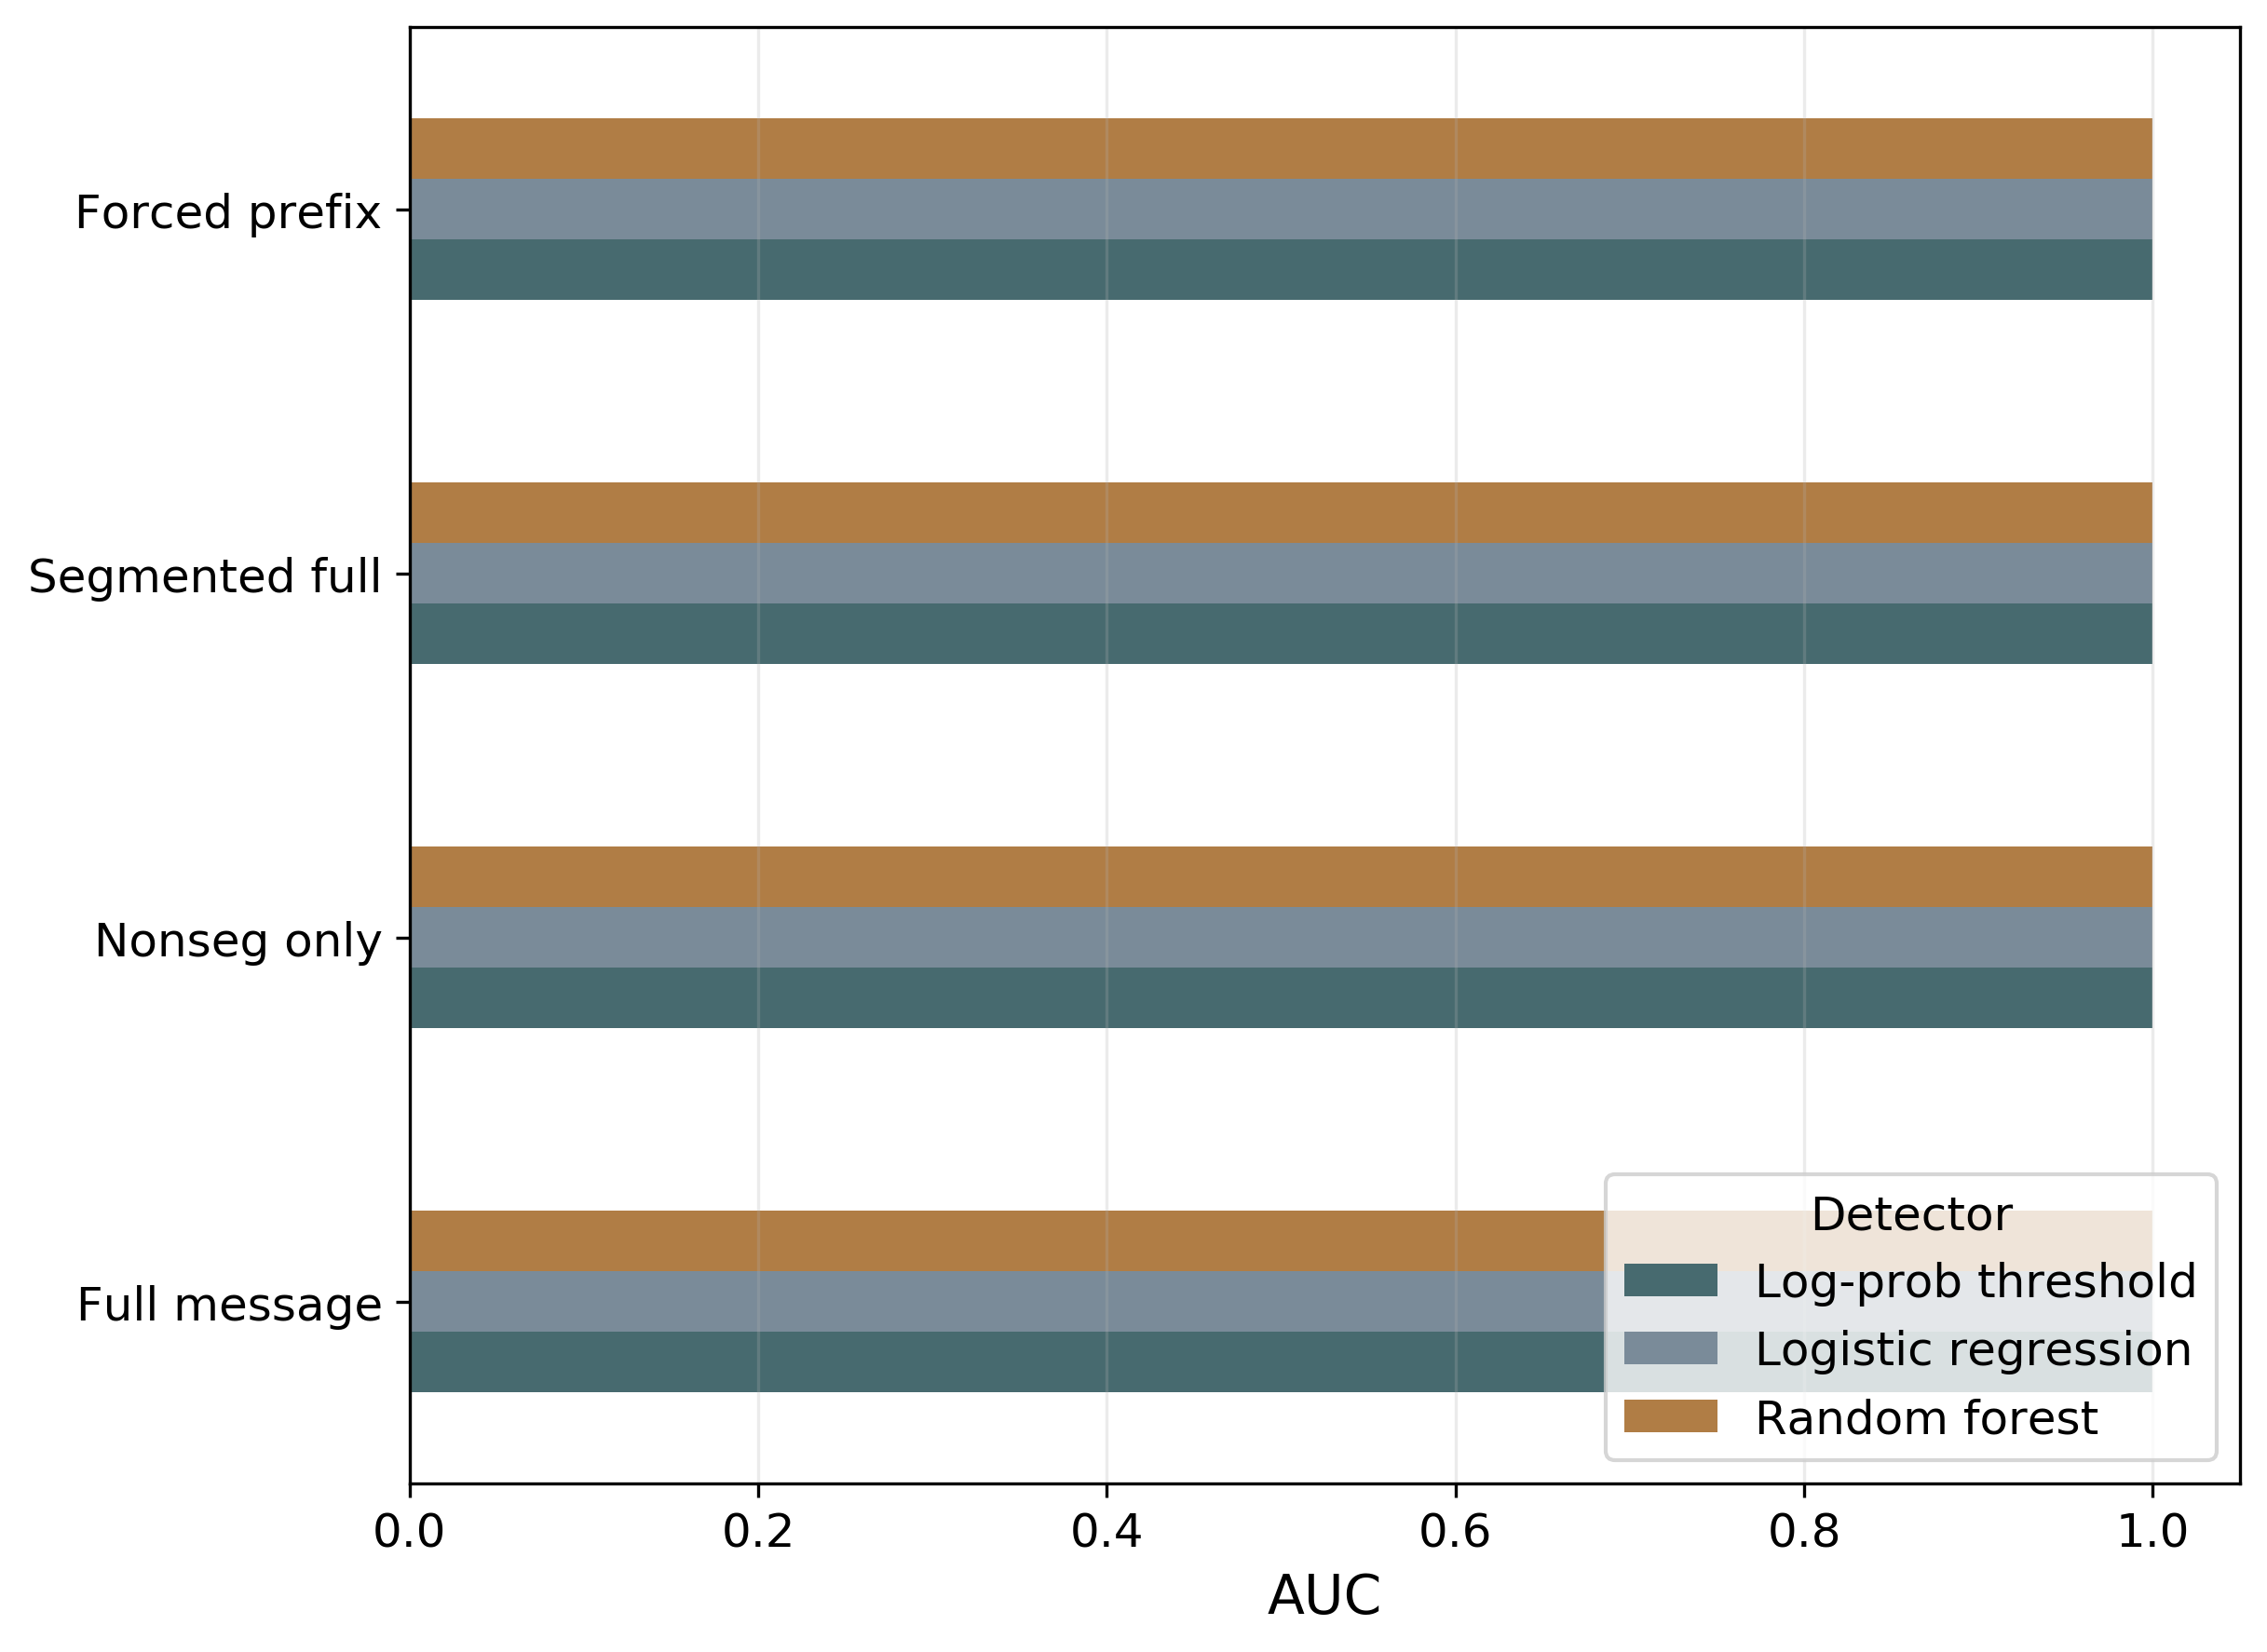
\includegraphics[width=0.95\linewidth]{figures/paper_detector_auc.png}
\caption{\label{fig:sdetector}Detector AUC summaries for the lightweight feature-only baselines. These results are based on the partial staged pilot and are treated as detector-pipeline checks rather than final steganalysis evidence.}
\end{figure}

The practical conclusion from Supplementary Figure~\ref{fig:sdetector} is that simple features can separate many of the completed rows in the current artifact package. This is useful for checking the detector pipeline and for motivating more careful steganalysis in future work. It should not be read as evidence that RankCloak is undetectable. The detector is feature-only, the sample is partial, and no raw-text detector or adversarial detector study is reported here.

Supplementary Figure~\ref{fig:seffects} summarizes selected effect-size estimates from the study. The purpose of this figure is to show which comparisons have the largest observed differences in the completed rows. These differences help explain which metrics are important enough to report in the main manuscript and which comparisons should be prioritized if the full matrix is later completed.

\begin{figure}[H]
\centering
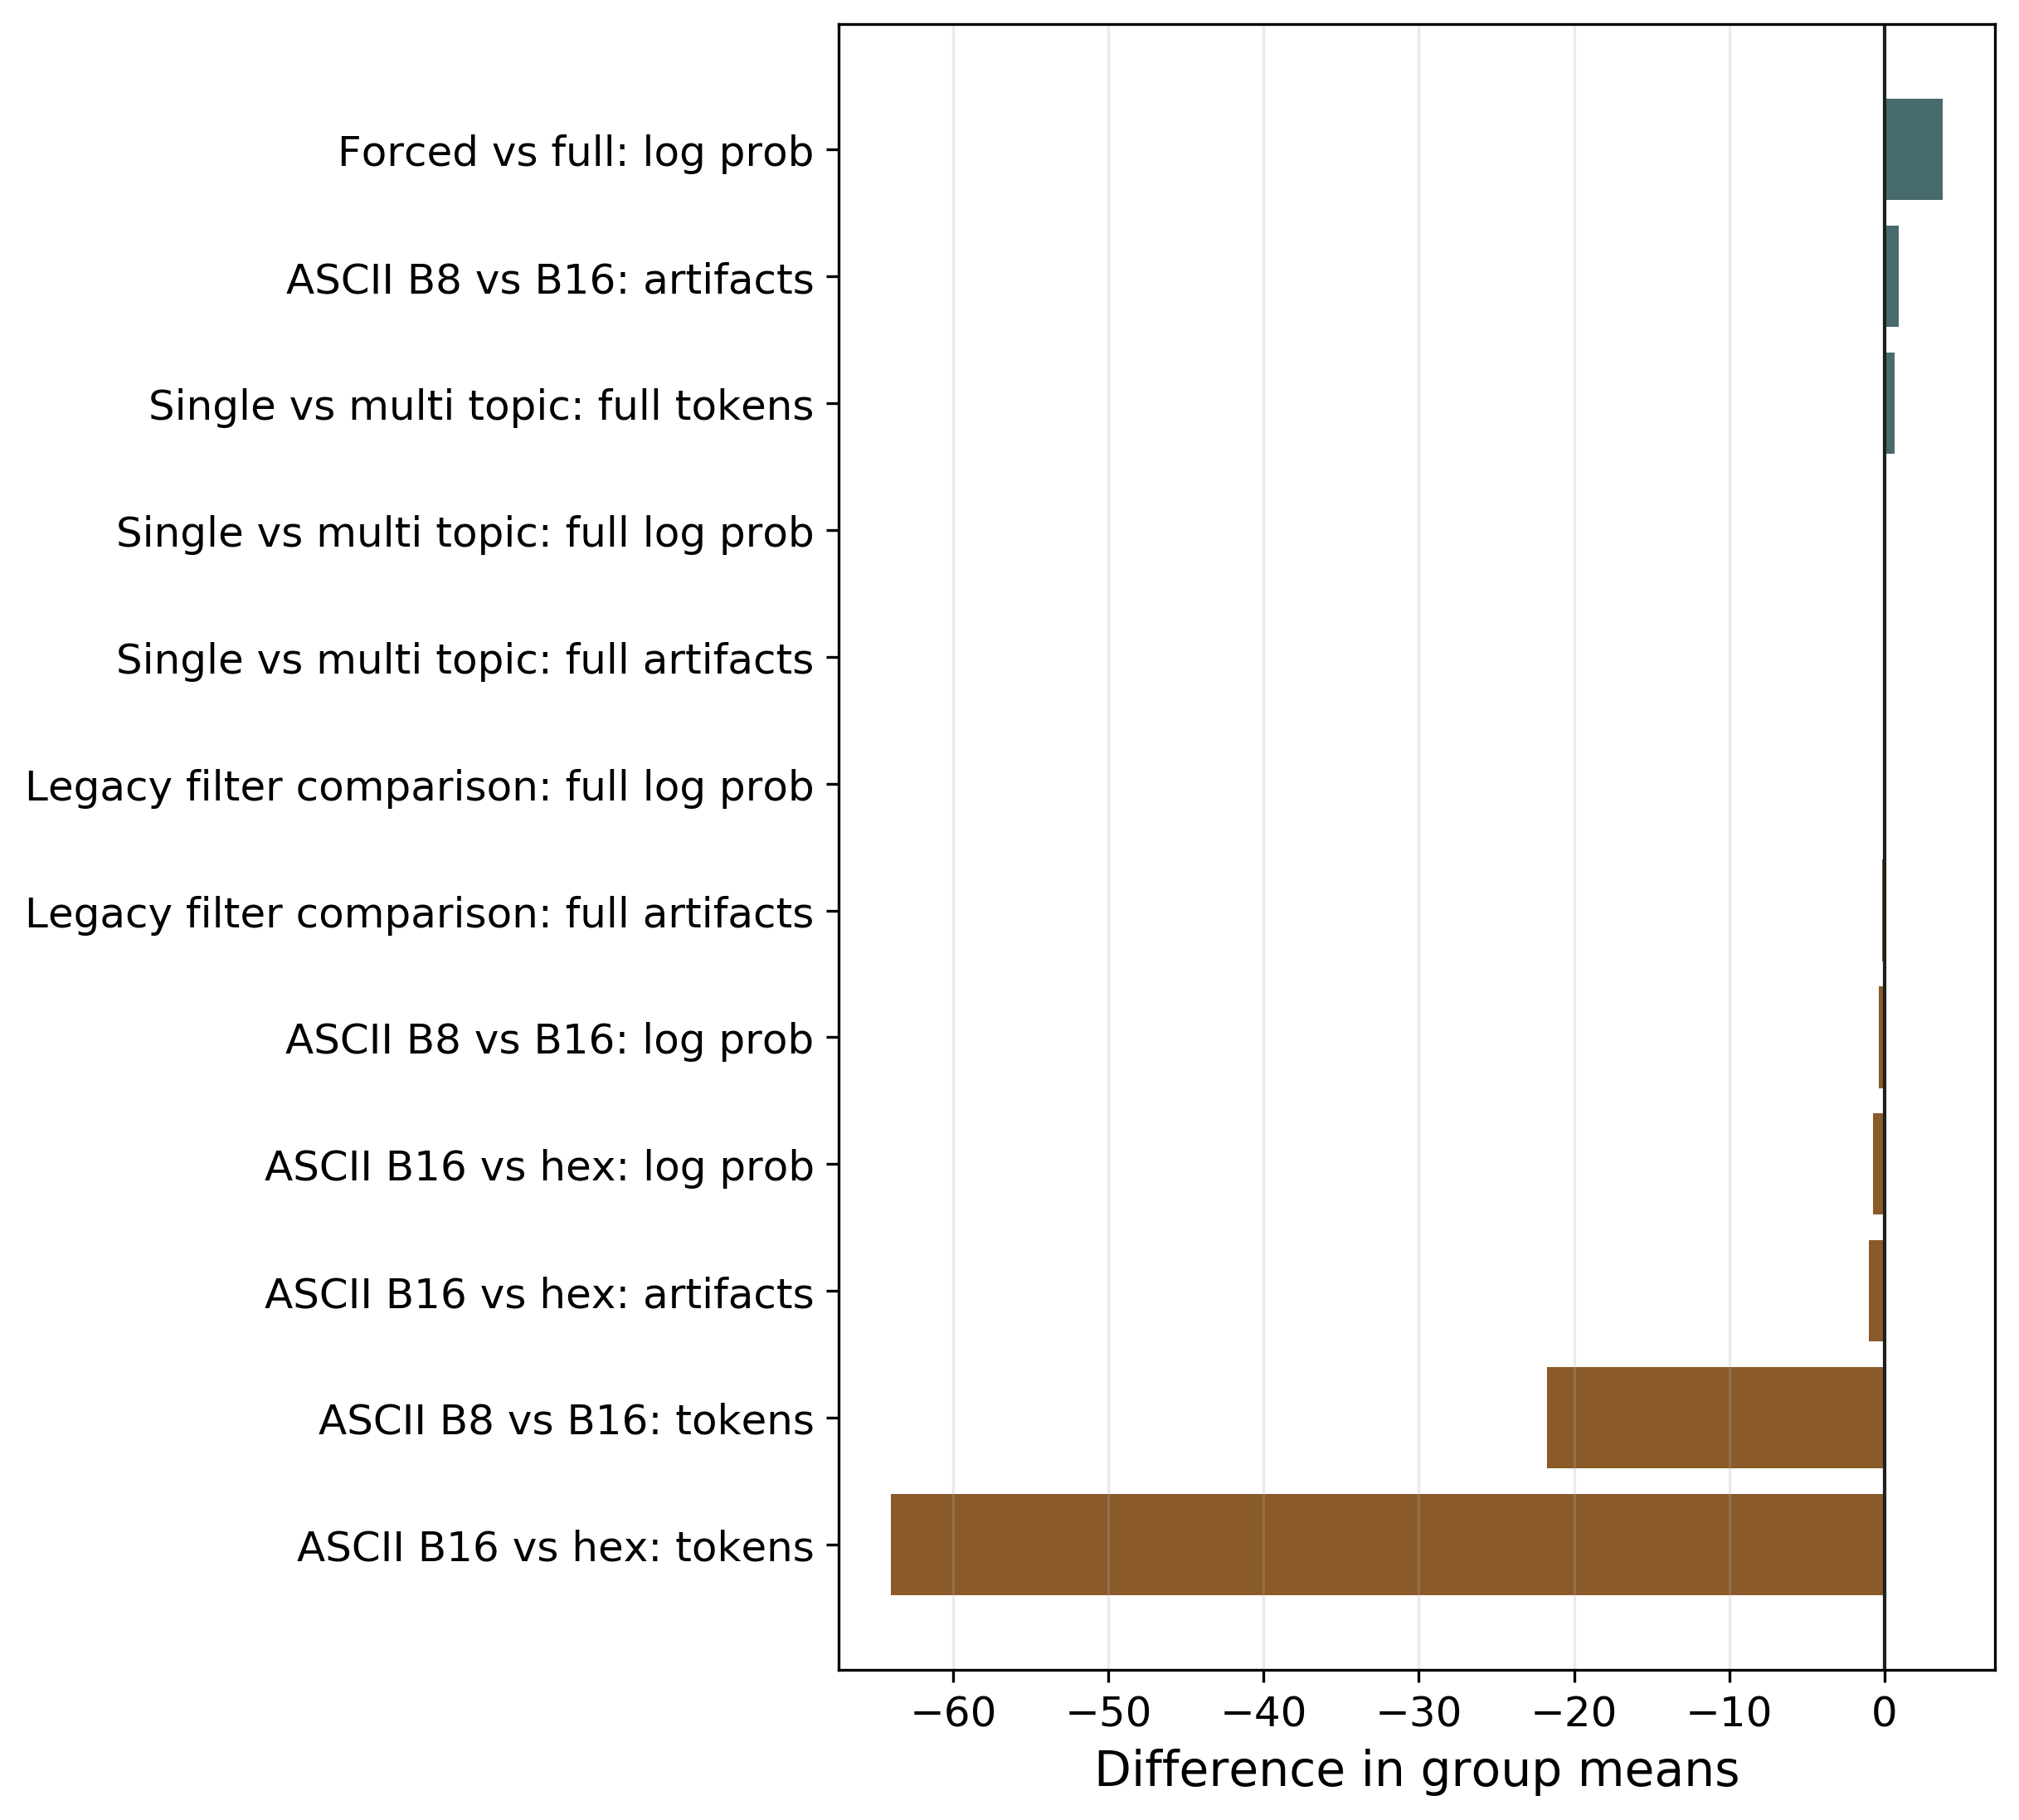
\includegraphics[width=0.95\linewidth]{figures/paper_effect_sizes_summary.png}
\caption{\label{fig:seffects}Effect-size summaries from the studys. Effect sizes are useful for planning and table structure, but the current matrix is incomplete.}
\end{figure}

Supplementary Figure~\ref{fig:seffects} should be read as a planning and interpretation aid. Large observed differences indicate where protocol choices, payload representations, or forced-span/full-message distinctions matter in the completed rows. They are not final inferential estimates because many planned paper-main rows remain incomplete.

Supplementary Figure~\ref{fig:sartifacts} reports deterministic artifact-flag counts by protocol variant. These flags capture simple visible patterns such as markup-like fragments, formatting artifacts, or other tracked string features. The purpose of the figure is to show where obvious generated-text artifacts were observed in the completed rows.

\begin{figure}[H]
\centering
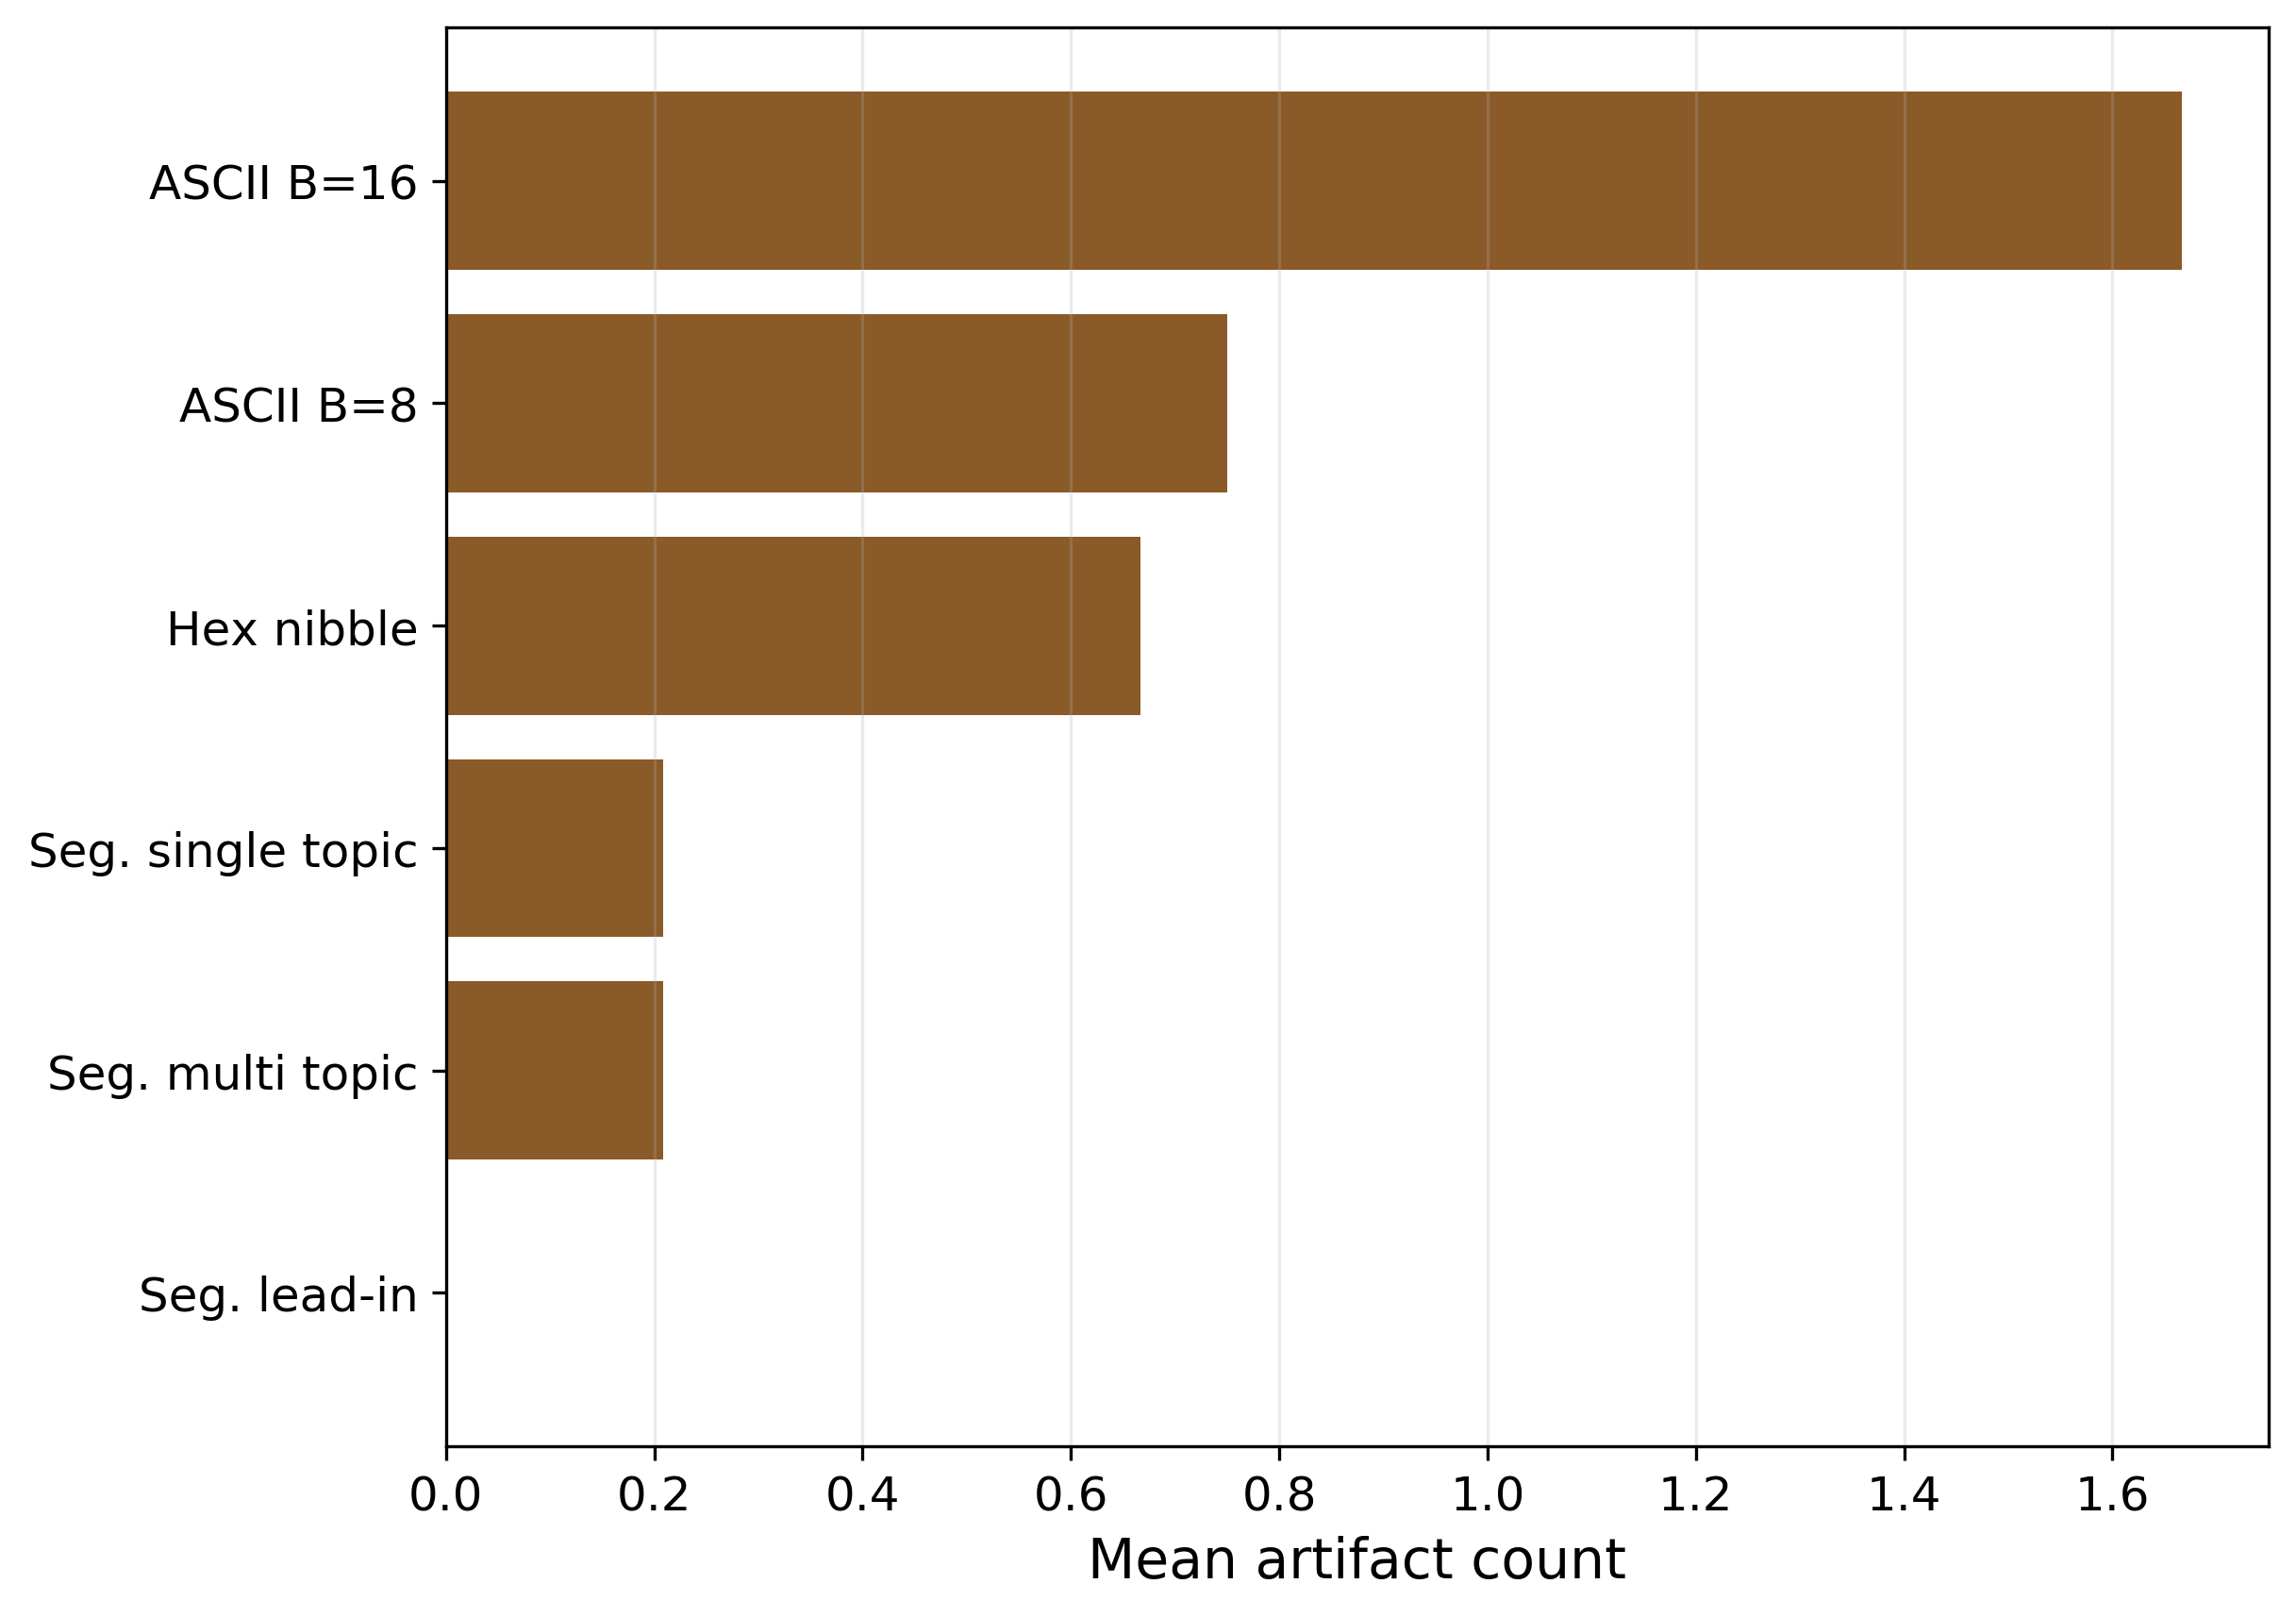
\includegraphics[width=0.95\linewidth]{figures/paper_artifact_counts_by_variant.png}
\caption{\label{fig:sartifacts}Artifact counts by variant for the current partial paper-main-pilot rows. Artifact flags are deterministic string-feature checks and do not replace human evaluation or steganalysis.}
\end{figure}

Supplementary Figure~\ref{fig:sartifacts} supports a limited conclusion. The tracked artifact flags are useful for auditing obvious formatting problems and for comparing protocol variants under a consistent feature rule. They are not a human naturalness score, and they do not establish detectability or undetectability. A row with few tracked artifacts may still be awkward to a human reader, and a row with more flags may still recover exactly.

Supplementary Figure~\ref{fig:sexploratory} summarizes earlier pilot studies that motivated the final paper-main design. Panel A focuses on fixed-rank alphabet stress: larger alphabets can reduce rank count but tend to lower the mean log-probability proxy. Panel B summarizes prompt-format pilots, showing that prompt engineering and dialogue-style prompts can change topic anchoring but do not by themselves solve forced-rank cover damage.

\begin{figure}[H]
\centering
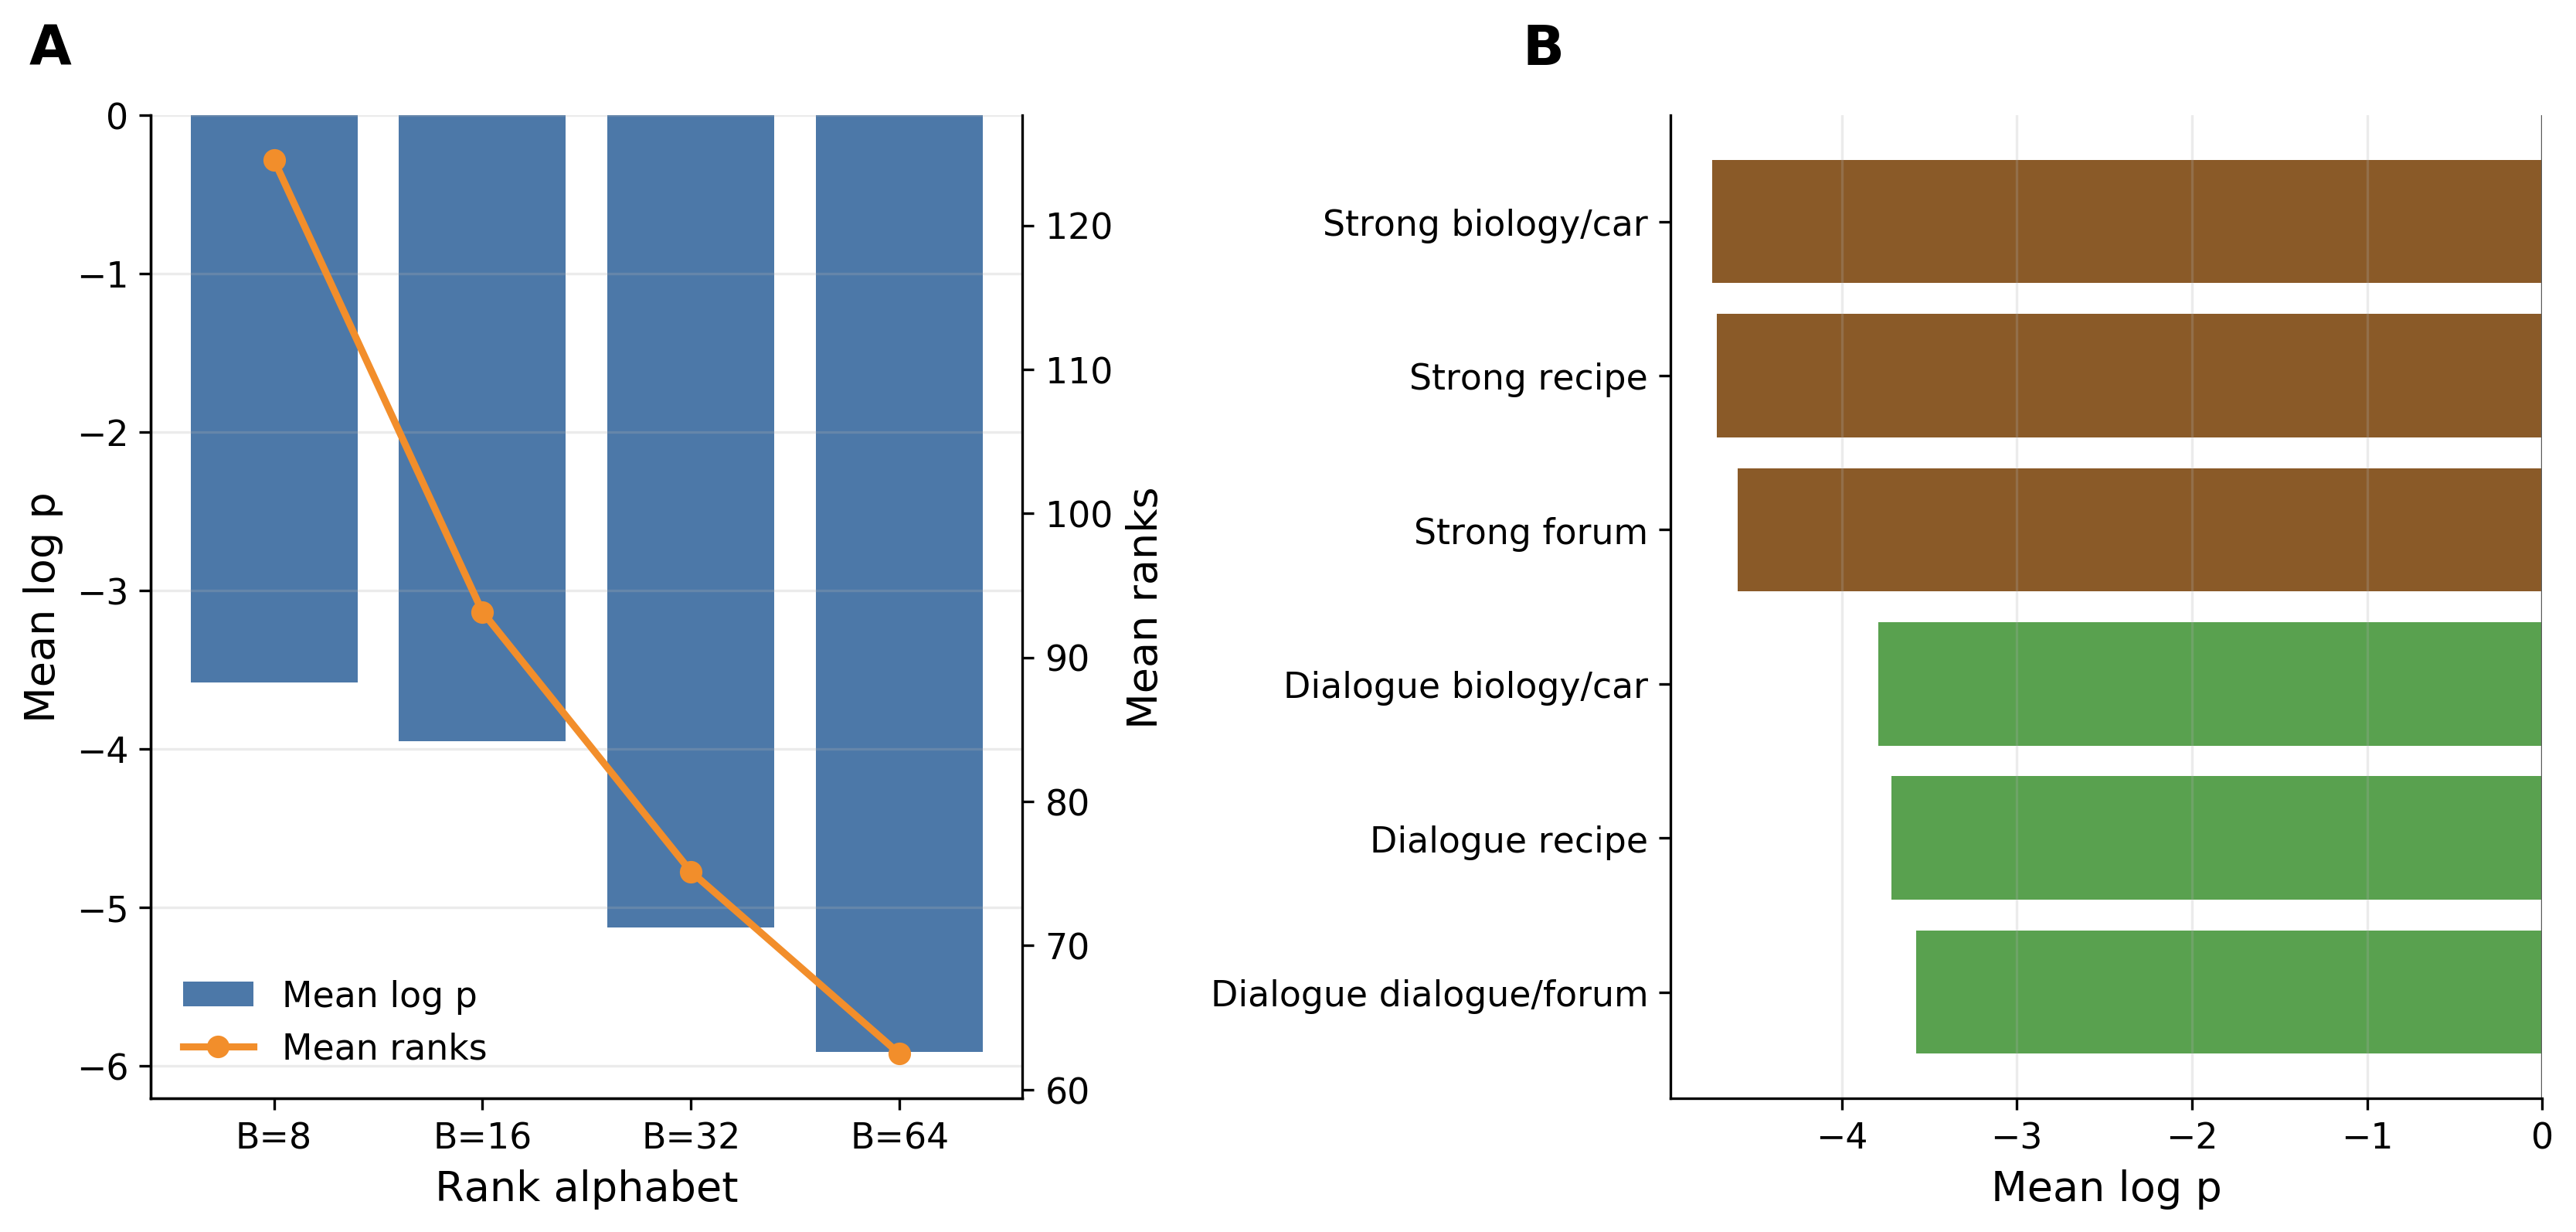
\includegraphics[width=0.95\linewidth]{figures/paper_exploratory_failure_modes.png}
\caption{\label{fig:sexploratory}Exploratory failure-mode diagnostics from earlier pilots. Panel A aggregates the small-full and strong-prompt sweeps, showing that larger fixed-rank alphabets shorten mean rank count while lowering the mean log-probability proxy. Panel B summarizes prompt-format pilot groups from the strong-prompt and dialogue-key pilots. These method-development results are not pooled into the paper-main inferential analysis and do not imply human naturalness or undetectability.}
\end{figure}

Supplementary Figure~\ref{fig:sexploratory} explains why the final paper-main-pilot focuses on bounded encodings, segmentation, natural tails, and filtering. The earlier pilots suggest that exact recovery can remain strong under exact-copy conditions, but public-message quality is sensitive to rank pressure, prompt format, and protocol structure. This is why the main manuscript treats RankCloak as a measurement framework: the important question is not only whether the payload can be recovered, but how each protocol choice changes cover-quality proxies and failure modes.






\end{document}
